       \documentclass[a4paper,12pt]{article}

    % With the commands after % signs you can define your own page size. Remove % to activate them and insert the values you want to define the size of the page you want.
    %\voffset=-2cm
    %\hoffset=-0.5cm
    %\textwidth=15cm
    %\parindent 0pt
    %\parskip 2ex
\usepackage{subfig}
\usepackage{color} 
\usepackage[usenames,dvipsnames,svgnames,table]{xcolor}

\usepackage[noindentafter]{titlesec}
\addtocounter{tocdepth}{1}  % Increase maximum TOC level by one
\addtocounter{secnumdepth}{1}  % Increase maximum section level by one

% Make paragraphs behave like subsubsections
\titleformat{\paragraph}[hang]{\sf\bfseries\normalfont\bf}{\thetitle\quad}{0pt}{}
\titlespacing{\paragraph}{0pt}{1em}{0.5em}

       \usepackage{graphicx}

\usepackage{multirow}
\usepackage{rotating}
\usepackage{chngpage}
\usepackage{amsmath}
\usepackage{listings}
\newcommand{\HRule}{\rule{\linewidth}{0.5mm}}
\usepackage{abstract}
\renewcommand{\abstractname}{}    % clear the title
\renewcommand{\absnamepos}{empty} % originally center




 \begin{document}
       \title{Global PID Framework Documentation}
        \author{Celeste Pidcott}
            \date{}
    \maketitle



%\tableofcontents

%\clearpage

%\listoffigures

%\listoftables

%\clearpage

%\begin{abstract}

%\end{abstract}


\section{Introduction}
\label{intro}

The global PID framework is designed to use sets of PID variables to 1) use MC data to create PDFs of these variables for a range of particle hypotheses, and 2) to use the PDFs as part of a log-likelihood method to determine the PID of reconstructed global tracks from data. The framework is designed such that new PID variables can be added as they are developed. Section 1 of this document will explain how to use the PID to produce PDFs, and how to perform PID on spill data contained within a Json document. Section 2 will detail how these two actions are performed within the code, and in Section 3 the PID variables, their structure, how new ones can be added to the framework, and details of those already in place, will be discussed. This document will be updated as the PID framework and variables continue to be developed.

\subsection{Using the PID scripts}
\label{use}

\subsection{Producing PDFs}
\label{PDFs}
Whilst the PID framework comes with PDFs provided in PIDhists.root, it is possible for a user to produce PDFs for hypotheses not included within this file. The following describes how this should be done.
\begin{figure}[h!]
\begin{center} 
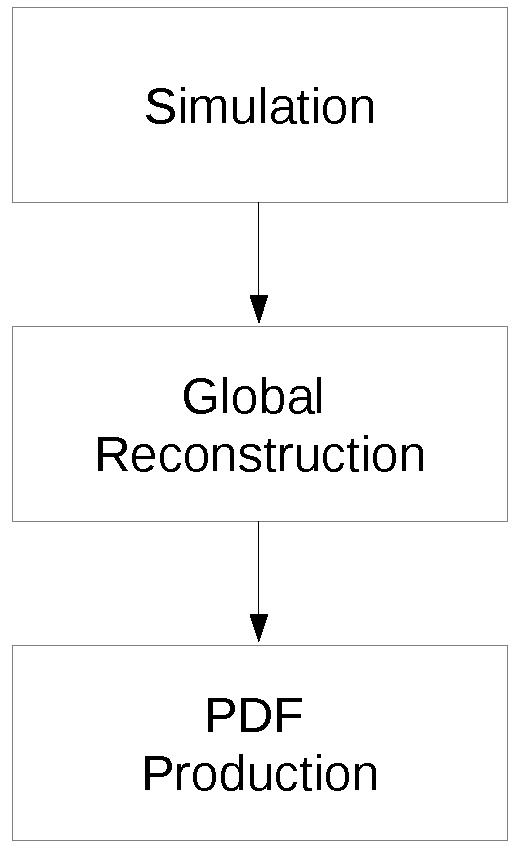
\includegraphics[width=2in]{pdfprodflow.pdf} 
\caption{Steps invloved in producing a PDF from MC data}
\label{pdfprod}
\end{center} 
\end{figure}
\begin{itemize}
\item Simulation: Production of MC data for a given particle 
hypothesis. To produce and output the MC to a Json file, a copy of 
simulate\_mice.py should be made, with the my\_output flag set to 
MAUS.OutputPyJSON().
\item Global Reconstruction: The MC data should then be passed through 
the global reconstruction. Detector information is currently added global tracks using the GlobalReconImport.py script in \\
\$\{MAUS\_ROOT\_DIR\}\textbackslash bin\textbackslash Global. This script calls the mapper 
MapCppGlobalReconImport, which constructs the global tracks required 
for the calculation of PID variables. The control variables to specify 
the input Json data sample, and the name of the output Json file that 
contains the reconstructed tracks can be set at the command line, or by 
using another datacard, as shown in listing ~\ref{globaldatacard}. To run 
the global reconstruction with the datacard, the following should be entered at the command line:

\begin{lstlisting}[breaklines=true,basicstyle=\ttfamily]
${MAUS_ROOT_DIR}/bin/Global/GlobalReconImport.py --configuration_file <name_of_datacard>
\end{lstlisting}

which for the example in ~\ref{globaldatacard} would be:

\begin{lstlisting}[breaklines=true,basicstyle=\ttfamily]
${MAUS_ROOT_DIR}/bin/Global/GlobalReconImport.py --configuration_file ex_global_datacard.py
\end{lstlisting}

\item PDF Production: To produce the PDFs from the reconstructed MC 
data, pid\_pdf\_production.py in \$\{MAUS\_ROOT\_DIR\}\textbackslash 
bin\textbackslash Global is then used. This script calls the reducer 
ReduceCppGlobalPID. With this script, a datacard, such as that shown 
given in listing ~\ref{pdfdatacard}, that includes the input Json filename, the global\_pid\_hypothesis for which the PDF(s) are to be produced, and a unique\_identifier (typically the time and date at which the script is run) is used by entering at the command line:
\begin{lstlisting}[breaklines=true,basicstyle=\ttfamily]
${MAUS_ROOT_DIR}/bin/Global/pid_pdf_generator.py --configuration_file example_pdf_datacard.py
\end{lstlisting}
This will create a directory within \$\{MAUS\_ROOT\_DIR\}\textbackslash files\textbackslash PID corresponding to the hypothesis and identifier given by the datacard, which will then contain files for each PID variable, each of which will contain the PDF for that hypothesis and variable.
\end{itemize}

\vspace*{1\baselineskip}

\begin{lstlisting}[language=Python,basicstyle=\ttfamily,frame=single,breaklines=true,commentstyle=\color{gray}, keywordstyle=\color{red}\bfseries,stringstyle=\color{green!50!black},captionpos=b,caption={An example datacard (ex\_global\_datacard.py) for use with GlobalReconImport.py},label=globaldatacard]
import os

# A json document containing spills from MC data
input_json_file_name = "example_hypothesis.json"
input_json_file_type = "text"

# The json document that the global tracks will be
# written to
output_json_file_name = 
	"example_hypothesis_Global_Recon.json"
output_json_file_type = "text"
\end{lstlisting}

\vspace*{2\baselineskip}

\begin{lstlisting}[language=Python,basicstyle=\ttfamily,frame=single,commentstyle=\color{gray}, breaklines=true,keywordstyle=\color{red}\bfseries,stringstyle=\color{green!50!black},captionpos=b,caption={An example datacard (example\_pdf\_datacard.py) for use with pid\_pdf\_generator.py},label=pdfdatacard]
import os
import datetime

# Use the current time and date as a unique
# identifier when creating files to contain PDFs. 
# A unique_identifier is required by the reducer, 
# and PDF production will fail without one.
now = datetime.datetime.now()
unique_identifier = 
	now.strftime("%Y_%m_%dT%H_%M_%S_%f")

# A json document containing global tracks from MC
# data
input_json_file_name = 
	"example_hypothesis_Global_Recon.json"
input_json_file_type = "text"

# The particle hypothesis that the PDF is being
# created for. A global_pid_hypothesis is required
# by the reducer, and PDF production will fail 
# without one.
global_pid_hypothesis = "example"
\end{lstlisting}

\subsubsection{Performing PID with pre-existing hypotheses}
\label{perf}
To perform PID on data, the steps shown figure ~\ref{pidperf} should be followed.

\begin{figure}[h!]
\begin{center} 
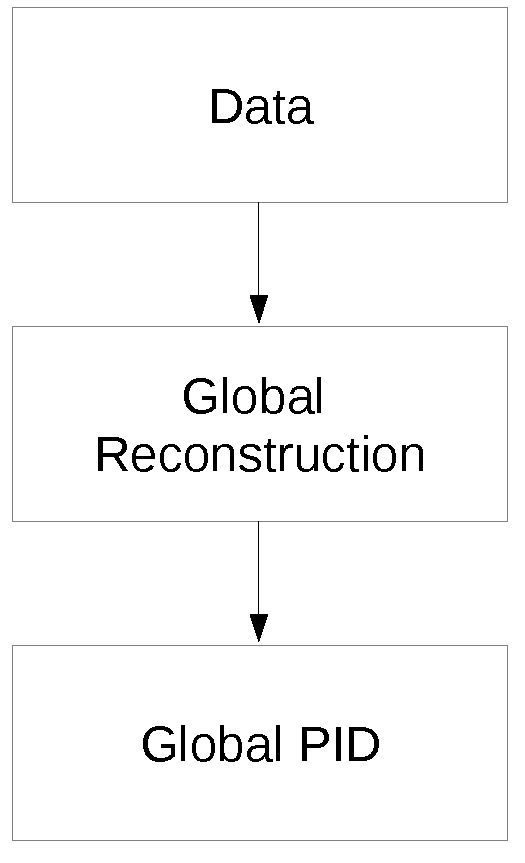
\includegraphics[width=2in]{pidperfflow.pdf} 
\caption{Steps invloved in performing the PID for a data sample}
\label{pidperf}
\end{center} 
\end{figure}
			
\begin{itemize}
\item Data: This can be experimental or MC data, however the spill data must be passed to the PID in a Json document.
\item Global Reconstruction: In the same way as described above, the 
data should then be passed through the global reconstruction, 
currently using the GlobalReconImport.py script in \$\{MAUS\_ROOT\_DIR\}\textbackslash 
bin\textbackslash Global, with a corresponding datacard containing the name of the input Json file and the name of the output file.
\item Global PID: To perform the PID on the reconstructed data, GlobalPID.py in \$\{MAUS\_ROOT\_DIR\}\textbackslash 
bin\textbackslash Global is then used. This script calls the 
MapCppGlobalPID mapper. With this script, a datacard, such as that 
shown given in listing ~\ref{piddatacard}, that includes the input and output Json filenames, is used, by entering the following at the command line:
\begin{lstlisting}[breaklines=true,basicstyle=\ttfamily]
${MAUS_ROOT_DIR}/bin/Global/GlobalPID.py 
	--configuration_file 
		example_pid_datacard.py
\end{lstlisting}
\end{itemize}

\begin{lstlisting}[language=Python,basicstyle=\ttfamily,breaklines=true,frame=single,commentstyle=\color{gray}, keywordstyle=\color{red}\bfseries,stringstyle=\color{green!50!black},captionpos=b,caption={An example datacard (example\_pid\_datacard.py) for use with GlobalPID.py},label=piddatacard]
import os

# A json document containing spills from data
input_json_file_name = 
	"example_hypothesis_Global_Recon.json"
input_json_file_type = "text"

# The json document that the global tracks will be
# written to
output_json_file_name = 
	"example_hypothesis_Global_PID.json"
output_json_file_type = "text"
\end{lstlisting}

As the framework currently stands, the output document would now contain the global tracks with the PID set (where it has been possible to do so) to whichever particle hypothesis had the highest log-likelihood. For tracks where the PID could not be determined, the track PID will be left as 0.

\section{MapCppGlobalPID and ReduceCppGlobalPID}
\label{mapred}
\subsection{MapCppGlobaPID}
\label{map}
The steps taken in MapCppGlobalPID for a single track are shown in 
figure \ref{mapflow}. To express this more fully, the data, having passed through the global reconstruction, is then passed to the PID. For each track, the values of each PID variable are calculated. Each of these values is then compared to the corresponding PDFs for all particle hypotheses, the number of entries in the corresponding bin providing the probability from which the log-likelihood is calculated. For each particle hypothesis, the log-likelihoods of all of the PID variables are summed to give a log-likelihood for that hypothesis. The PID of the track is then obtained by comparing the log-likelihoods of the hypotheses.
\begin{figure}[h!]
\begin{center} 
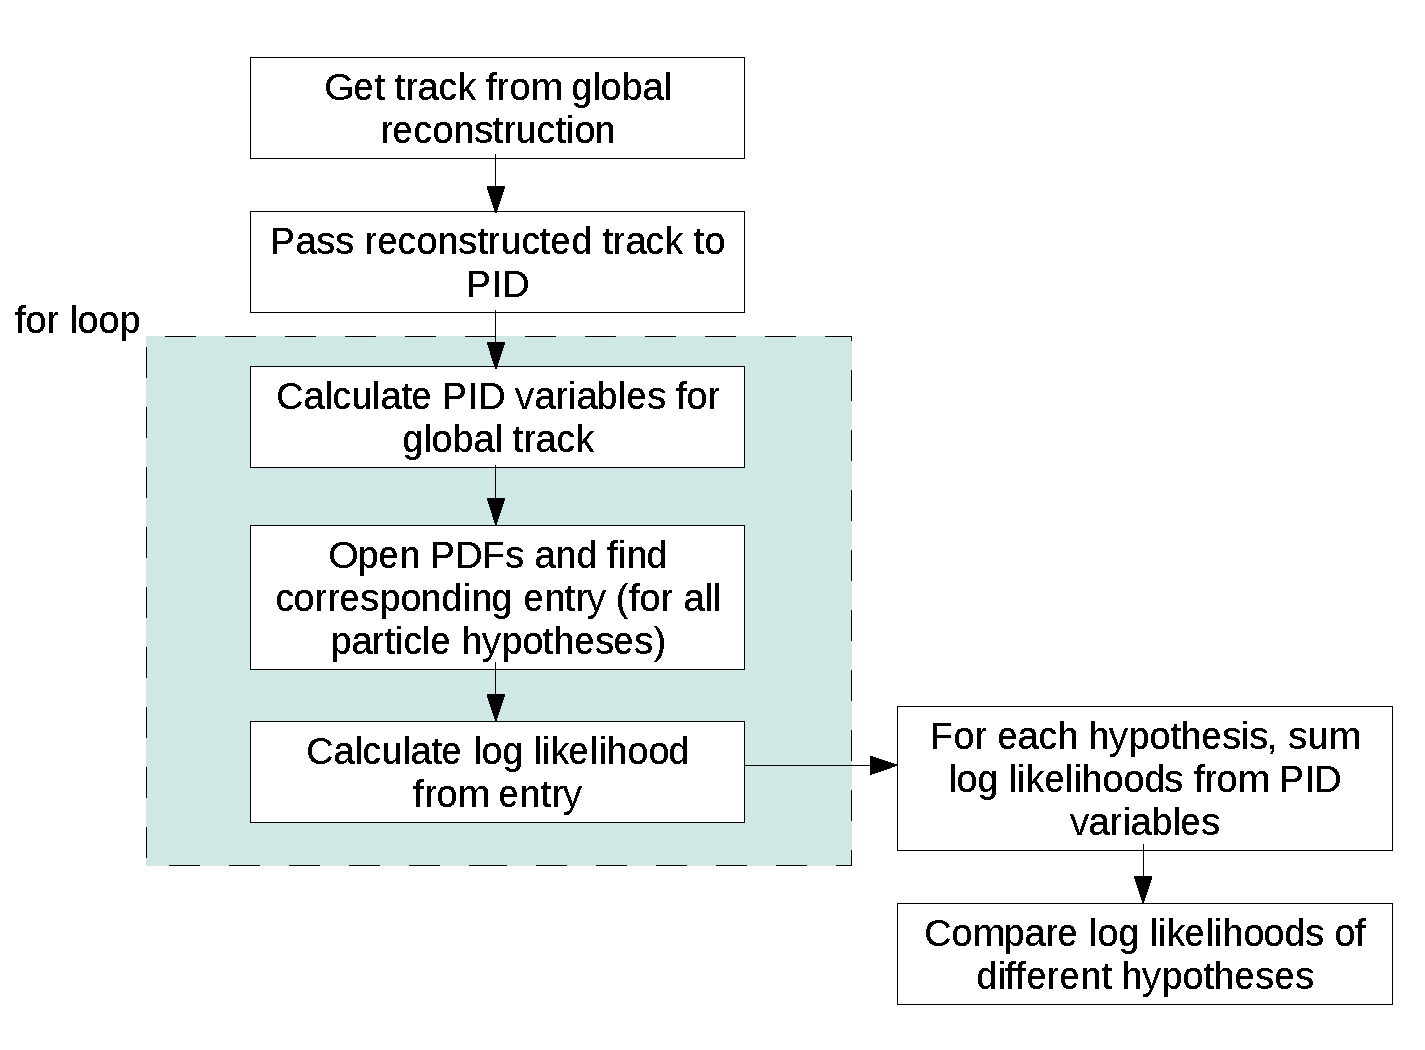
\includegraphics[width=5in]{PIDflow.pdf} 
\caption{Flow chart detailing steps taken in MapCppGlobaPID}
\label{mapflow}
\end{center} 
\end{figure}

\section{ReduceCppGlobalPID}
\label{reducer}
The steps taken in ReduceCppGlobalPID are shown in figure ~\ref{reduceflow}. MC data for a given particle hypothesis, having passed through the global reconstruction, is then passed to the PID. For each track, the values of each PID variable are calculated. A histogram is filled with these values. If the behaviour has been turned on in the PID variable class, then a single event is spread over all bins in the histogram, to ensure that when the PDF is used by the PID, there will no empty bins, thus avoiding cases where the log-likelihood takes the log of zero. The histogram is then normalised to create the PDF, which is then written and saved to file.
If a MC track returns a variable value outside of the allowed range of the histogram (as defined within the variable class) then the value for that track is not included.
\begin{figure}[h!]
\begin{center} 
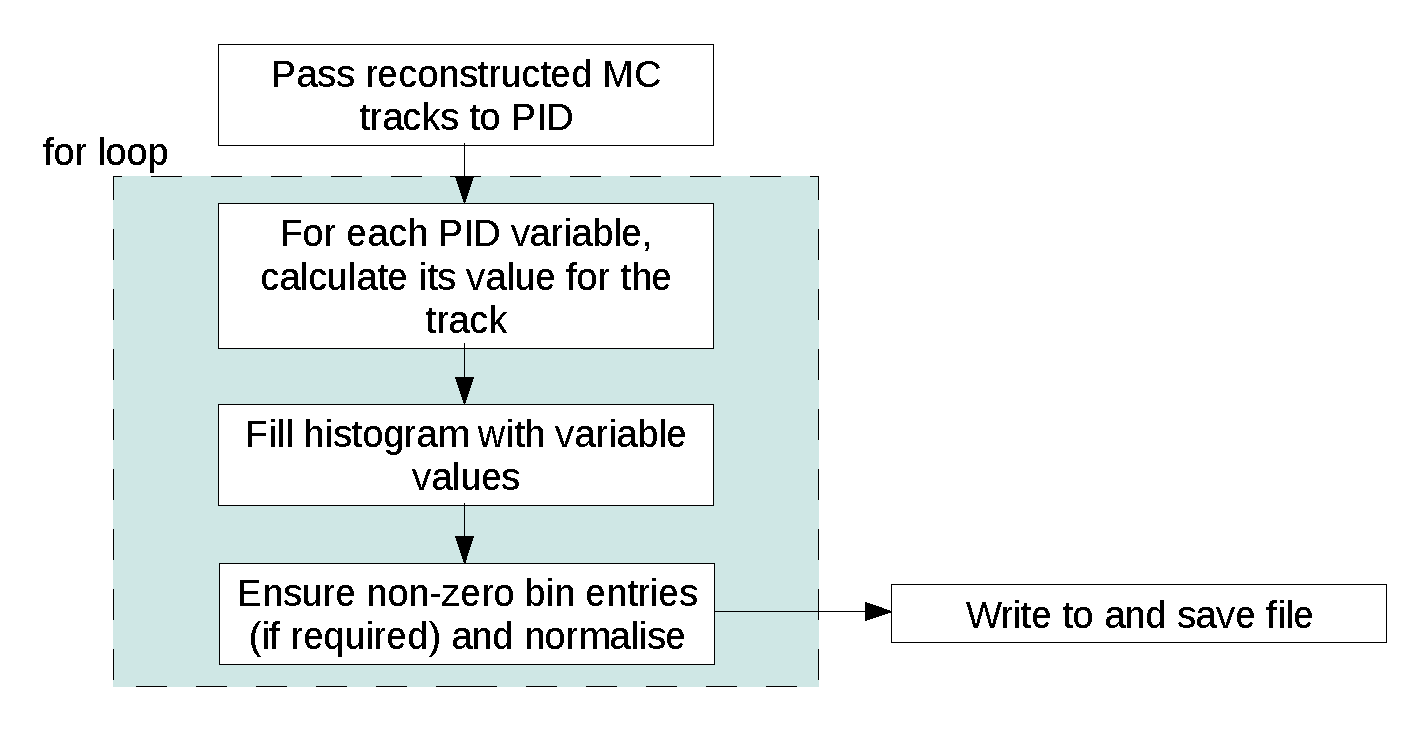
\includegraphics[width=5in]{PDFflow.pdf} 
\caption{Flow chart detailing steps taken in ReduceCppGlobaPID}
\label{reduceflow}
\end{center} 
\end{figure}

\section{PID Variables}
\label{PID}
Information from the MICE detectors will be incorporated into a set of 
PID variables that can be used to distinguish between particle 
hypotheses.
The Global PID framework has been written such that any number of PID 
variables can be developed and added as necessary, all represented by 
their own class, derived from a base class.

\subsection{PID Base Class}
\label{PIDBase}
The base PID class (PIDBase.hh and .cc) contains the functions to:
\begin{itemize}
\item Create the PDFs (and the files that contain them)
\item Use the PDFs with globally reconstructed tracks
\item Populate the PDFs with variable values (after checking that 
value is valid)
\item Perform the log-likelihood for an incoming globally reconstructed 
track (after checking that value of variable for track falls within 
range of PDF).
\item Calculate the value of the PID variable (this is a virtual 
function to be defined in the derived classes)
\end{itemize}

\subsection{PID Variable Classes}
\label{PIDVar}
Each PID variable will be implemented in a derived class of the base PID class. Because of how the framework is designed, new variables can be added as they are developed.

\subsubsection{Adding PID Variables}
\label{addvar}
In each derived variable class, the following should be included:
\begin{itemize}
\item The variable name should be set
\item The function to calculate the PID variable should be defined.  
\item The minimum, maximum, and number of bins for PDFs created using 
the variable should be set. The values of the minimum and maximum 
define the allowed range of values that the PID variable can take.
\item In some cases it may be necessary to ensure that all bins in a 
PDF return non zero entries, and so by setting the variable 
\_nonZeroHistEntries to true, a single event spread accross all bins 
will be added
\end{itemize}

\subsubsection{PIDVarA}
\label{PIDVarA}
There is currently a single PID variable defined within the framework, 
PIDVarA (see PIDVarA.hh and .cc), which uses the difference between the times measured at TOF1 
and TOF0 as its variable. Only for tracks where there is a single TOF0 
and a single TOF1 time measurement, and for which the time difference 
between the detectors falls within the minimum and maximum set within 
the class, will a valid value of the variable be returned. Otherwise, 
the value of the variable is set to -1, such that it falls outside of 
the allowed range for the variable, and so variable for the track is 
not used in PDF production, or in the PID.

\clearpage

%\begin{thebibliography}{99}

%\end{thebibliography}



\end{document}
